\documentclass[border=6pt]{standalone}
\usepackage{tikz}
\usepackage[edges]{forest}
\usetikzlibrary{arrows.meta,positioning,calc,decorations.pathreplacing,shapes.geometric}
\begin{document}
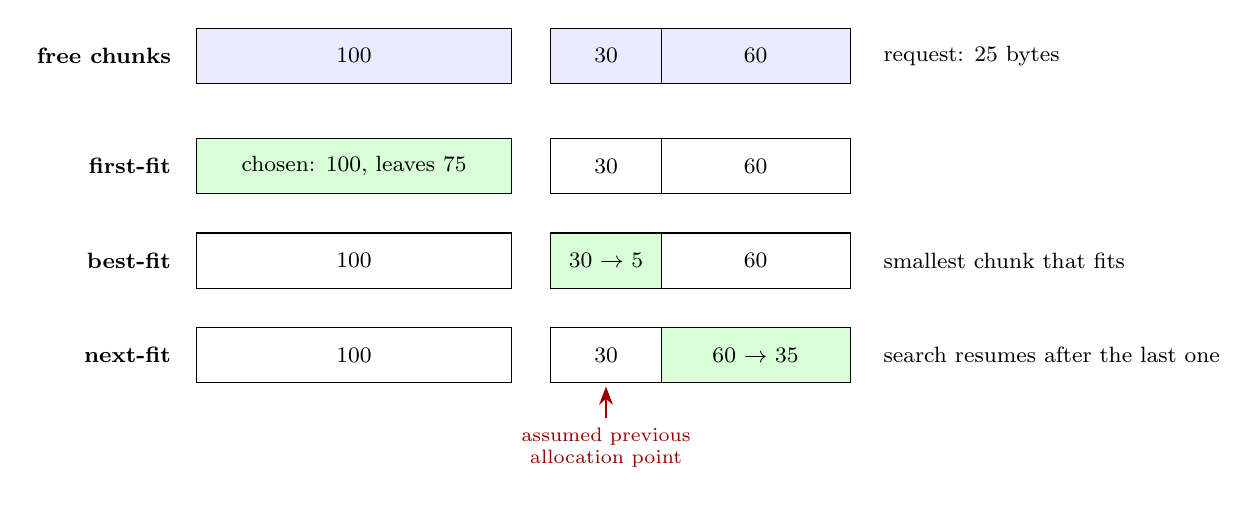
\begin{tikzpicture}[>=Stealth,font=\small,
 ch/.style={draw,minimum height=0.7cm,align=center,font=\footnotesize}]
\node[font=\footnotesize\bfseries,anchor=east] at (-0.2,1.9) {free chunks};
\node[ch,minimum width=4.0cm,fill=blue!8] (a) at (2.0,1.9) {100};
\node[ch,minimum width=1.4cm,fill=blue!8] (b) at (5.2,1.9) {30};
\node[ch,minimum width=2.4cm,fill=blue!8] (c) at (7.1,1.9) {60};
\node[font=\footnotesize,anchor=west] at (8.6,1.9) {request: 25 bytes};
\node[font=\footnotesize\bfseries,anchor=east] at (-0.2,0.5) {first-fit};
\node[ch,minimum width=4.0cm,fill=green!15] at (2.0,0.5) {chosen: 100, leaves 75};
\node[ch,minimum width=1.4cm] at (5.2,0.5) {30}; \node[ch,minimum width=2.4cm] at (7.1,0.5) {60};
\node[font=\footnotesize\bfseries,anchor=east] at (-0.2,-0.7) {best-fit};
\node[ch,minimum width=4.0cm] at (2.0,-0.7) {100};
\node[ch,minimum width=1.4cm,fill=green!15] at (5.2,-0.7) {30 $\to$ 5}; \node[ch,minimum width=2.4cm] at (7.1,-0.7) {60};
\node[font=\footnotesize,anchor=west] at (8.6,-0.7) {smallest chunk that fits};
\node[font=\footnotesize\bfseries,anchor=east] at (-0.2,-1.9) {next-fit};
\node[ch,minimum width=4.0cm] at (2.0,-1.9) {100};
\node[ch,minimum width=1.4cm] at (5.2,-1.9) {30}; \node[ch,minimum width=2.4cm,fill=green!15] at (7.1,-1.9) {60 $\to$ 35};
\draw[->,thick,red!60!black] (5.2,-2.7) node[below,font=\scriptsize,align=center]{assumed previous\\allocation point} -- (5.2,-2.3);
\node[font=\footnotesize,anchor=west] at (8.6,-1.9) {search resumes after the last one};
\end{tikzpicture}
\end{document}
